\documentclass[preprint, 3p,
authoryear]{elsarticle} %review=doublespace preprint=single 5p=2 column
%%% Begin My package additions %%%%%%%%%%%%%%%%%%%

\usepackage[hyphens]{url}

  \journal{Passion Papillon} % Sets Journal name

\usepackage{graphicx}
%%%%%%%%%%%%%%%% end my additions to header

\usepackage[T1]{fontenc}
\usepackage{lmodern}
\usepackage{amssymb,amsmath}
% TODO: Currently lineno needs to be loaded after amsmath because of conflict
% https://github.com/latex-lineno/lineno/issues/5
\usepackage{lineno} % add
\usepackage{ifxetex,ifluatex}
\usepackage{fixltx2e} % provides \textsubscript
% use upquote if available, for straight quotes in verbatim environments
\IfFileExists{upquote.sty}{\usepackage{upquote}}{}
\ifnum 0\ifxetex 1\fi\ifluatex 1\fi=0 % if pdftex
  \usepackage[utf8]{inputenc}
\else % if luatex or xelatex
  \usepackage{fontspec}
  \ifxetex
    \usepackage{xltxtra,xunicode}
  \fi
  \defaultfontfeatures{Mapping=tex-text,Scale=MatchLowercase}
  \newcommand{\euro}{€}
\fi
% use microtype if available
\IfFileExists{microtype.sty}{\usepackage{microtype}}{}
\usepackage[]{natbib}
\bibliographystyle{elsarticle-harv}

\usepackage{graphicx}
\ifxetex
  \usepackage[setpagesize=false, % page size defined by xetex
              unicode=false, % unicode breaks when used with xetex
              xetex]{hyperref}
\else
  \usepackage[unicode=true]{hyperref}
\fi
\hypersetup{breaklinks=true,
            bookmarks=true,
            pdfauthor={},
            pdftitle={Dynamiques spatio-temporelles des lépidoptères au Québec (1859--2023)},
            colorlinks=false,
            urlcolor=blue,
            linkcolor=magenta,
            pdfborder={0 0 0}}

\setcounter{secnumdepth}{5}
% Pandoc toggle for numbering sections (defaults to be off)


% tightlist command for lists without linebreak
\providecommand{\tightlist}{%
  \setlength{\itemsep}{0pt}\setlength{\parskip}{0pt}}







\begin{document}


\begin{frontmatter}

  \title{Dynamiques spatio-temporelles des lépidoptères au Québec
(1859--2023)}
    \author[Université de Sherbrooke]{Maxence Comyn%
  %
  }
   \ead{comm2008@usherbrooke.ca} 
    \author[Université de Sherbrooke]{Félix Laberge%
  %
  }
   \ead{flix.laberge2@usherbrooke.ca} 
    \author[Université de Sherbrooke]{Julianne Lemay-St-Laurent%
  %
  }
   \ead{lemj2221@usherbrooke.ca} 
    \author[Université de Sherbrooke]{Elsa Michel%
  %
  }
   \ead{elsa.michel@usherbrooke.ca} 
      \affiliation[Département de biologie de l'université de
Sherbrooke]{
    organization={Université de Sherbrooke},addressline={2500 Boulevard
Université},city={Sherbrooke},postcode={J1K
2R1},state={Québec},country={Canada},}
    \cortext[cor1]{Corresponding author}
  
  \begin{abstract}
  Ce projet s'intéresse aux variations temporelles et spatiales des
  lépidoptères au Québec à partir d'observations récoltés entre 1859 et
  2023. Des analyses ont permis d'étudier le nombre d'espèces observées,
  pour la première et la dernière fois par décennie, leur répartition
  selon la latitude et la localisation des observations. Les dernières
  décennies présentent davantage d'observations et d'espèces vues pour
  la première et la dernière fois. Ces résultats s'expliquent par un
  déclin possible d'espèces et un échantillonnage plus intensif, grâce à
  l'avancée scientifique. Puisque la température y est plus élevée, le
  sud du Québec montre une plus grande richesse spécifique.
  L'utilisation de données issues de la science citoyenne introduit
  certains biais, concernant les préférences de la population et le fait
  qu'elle est plus dense au sud.
  \end{abstract}
  
 \end{frontmatter}

\section{Introduction}\label{introduction}

Les insectes sont grandement impactés par l'activité humaine et ce qui
en découle, comme les changements climatiques. L'exploration du monde
vivant, tout en exerçant une pression sur la biodiversité, est aussi un
levier essentiel pour mieux la comprendre et la préserver. Dans ce
contexte, la science citoyenne est une bonne façon de récolter beaucoup
de données à moindres coûts. Une partie des données utilisées pour ce
projet provient justement d'initiatives de science citoyenne. Bien que
les insectes jouent un rôle écologique majeur, ils demeurent globalement
sous-représentés dans la littérature scientifique. Du moins, parmi tous
les taxons d'insectes, les lépidoptères sont les plus étudiés {[}1{]}.
Il est alors pertinent de se demander comment la structure des
communautés de papillons varie au niveau temporel et spatial au Québec.
Des analyses ont été faites afin d'identifier combien d'espèces ont été
observées pour la première et la dernière fois pendant chaque décennie
pour les années où les données ont été récoltées. Des graphiques ont
ensuite été conçus pour déterminer à quelles latitudes se retrouvent le
plus d'espèces. Finalement, une carte des observations a été créée pour
illustrer où elles sont localisées.

\begin{center}\rule{0.5\linewidth}{0.5pt}\end{center}

\section{Méthodes}\label{muxe9thodes}

Un jeu de données de plus de 400 000 observations ponctuelles a été
analysé avec le logiciel R {[}2{]}. Ces observations proviennent de
différentes sources et ont été échantillonnées entre les années 1859 à
2023. Les fichiers ont été fusionnés à l'aide de la librairie
data.table\_1.17.0 {[}3{]}. Le tout a ensuite été nettoyé avec
dplyr\_1.1.4{[}4{]}. Pour faire les tables avec le langage SQL, la
librairie RSQLite\_2.3 {[}5{]} fut utilisée. Les données ont été
analysées en ne conservant que celles comprises dans la géographie du
Québec (de latitude entre 44 et 66 degrés et de longitude allant de -80
à -57 degrés). Des figures ont été faites pour visualiser le nombre
d'espèces par décennie (vues pour la première fois, la dernière fois et
observées au total). Ces données ont été regroupées par décennies pour
simplifier la visualisation, considérant que, durant les premières
années, peu d'activité a été reportée. Cependant, les décennies 1860,
1870 et 2020 ne comportent pas 10 ans de données contrairement aux
autres. Par exemple, il n'y a pas de données concernant 1870 ou 1871. De
plus, la décennie 2020 n'a pas été prise en compte pour l'analyse
puisqu'il est normal que les dernières observations de ces espèces
soient pendant les dernières années de la base de données.

Pour analyser les variations spatiales, un graphique du nombre d'espèces
par latitude a été fait, accompagné d'une carte localisant les
observations. Nous avons eu recours aux librairies leaflet\_2.2.2
{[}6{]} et ggplot2\_3.5.1{[}7{]} pour réaliser ces figures et la carte.
La librairie targets {[}8{]} fut utilisée pour rendre le processus plus
efficace par un pipeline.

\section{Résultats}\label{ruxe9sultats}

Comme le montre la figure 1, la décennie qui présente le plus grand
nombre d'espèces, soit 2034 espèces, est celle de 2020. Le nombre
d'espèces observées pour la première fois était supérieur dans la
décennie 2000, soit 1366 espèces (figure 2). Au total, 506 et 459
espèces ont été vues pour la dernière fois respectivement durant les
décennies 2010 puis 2000, ce qui est plus élevé que pour les autres
années (figure 3). Comme présenté par la figure 4, la majorité des
données proviennent du 21e siècle. En effet, 42 411 observations ont été
collectées de 1860 à 1999 alors que 233 214 observations ont été
reportées de 2000 à 2023. La figure 5 montre que les espèces de
lépidoptères sont plus nombreuses au sud, plus précisément entre les
latitudes de 44 à 49.5 degrés. Peu ont été reportées au nord. La carte
de la figure 6 illustre la position des observations reportées.

\begin{center}\rule{0.5\linewidth}{0.5pt}\end{center}

\begin{figure}
\centering
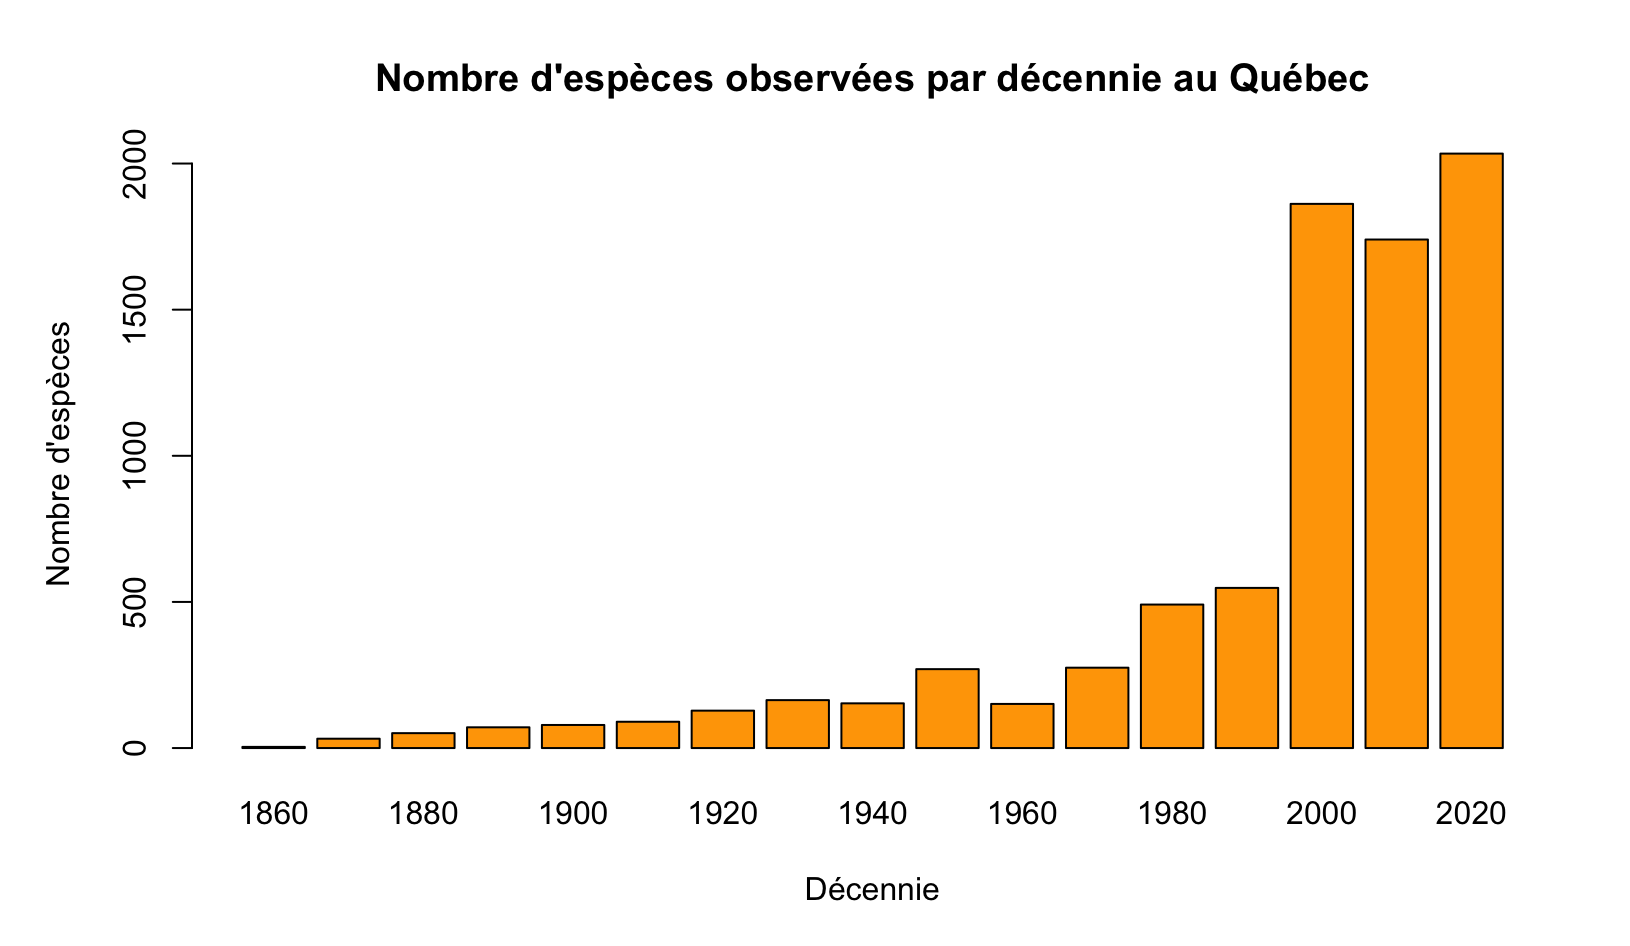
\includegraphics[width=\textwidth,height=0.4\textheight]{nb_esp_obs_par_decennie.png}
\caption{Nombre d'espèces de papillons observées par décennie au Québec}
\end{figure}

\begin{figure}
\centering
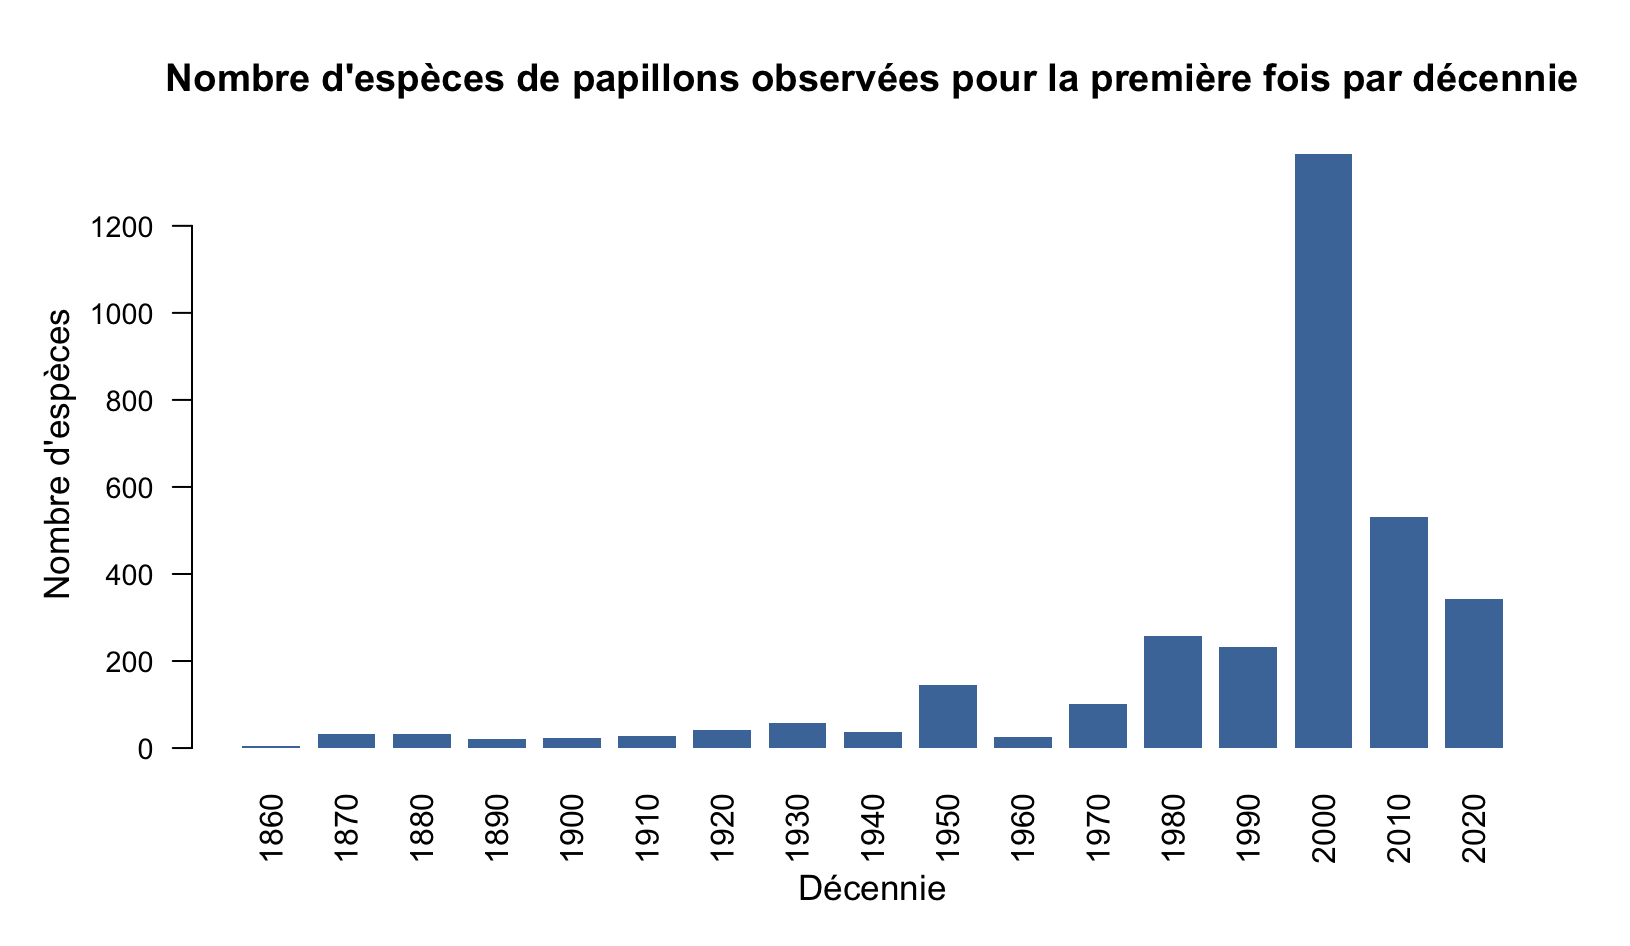
\includegraphics[width=\textwidth,height=0.4\textheight]{fig_nb_esp_obs_premiere_fois.png}
\caption{Nombre d'espèces de papillons observées pour la première fois
par décennie au Québec}
\end{figure}

\begin{figure}
\centering
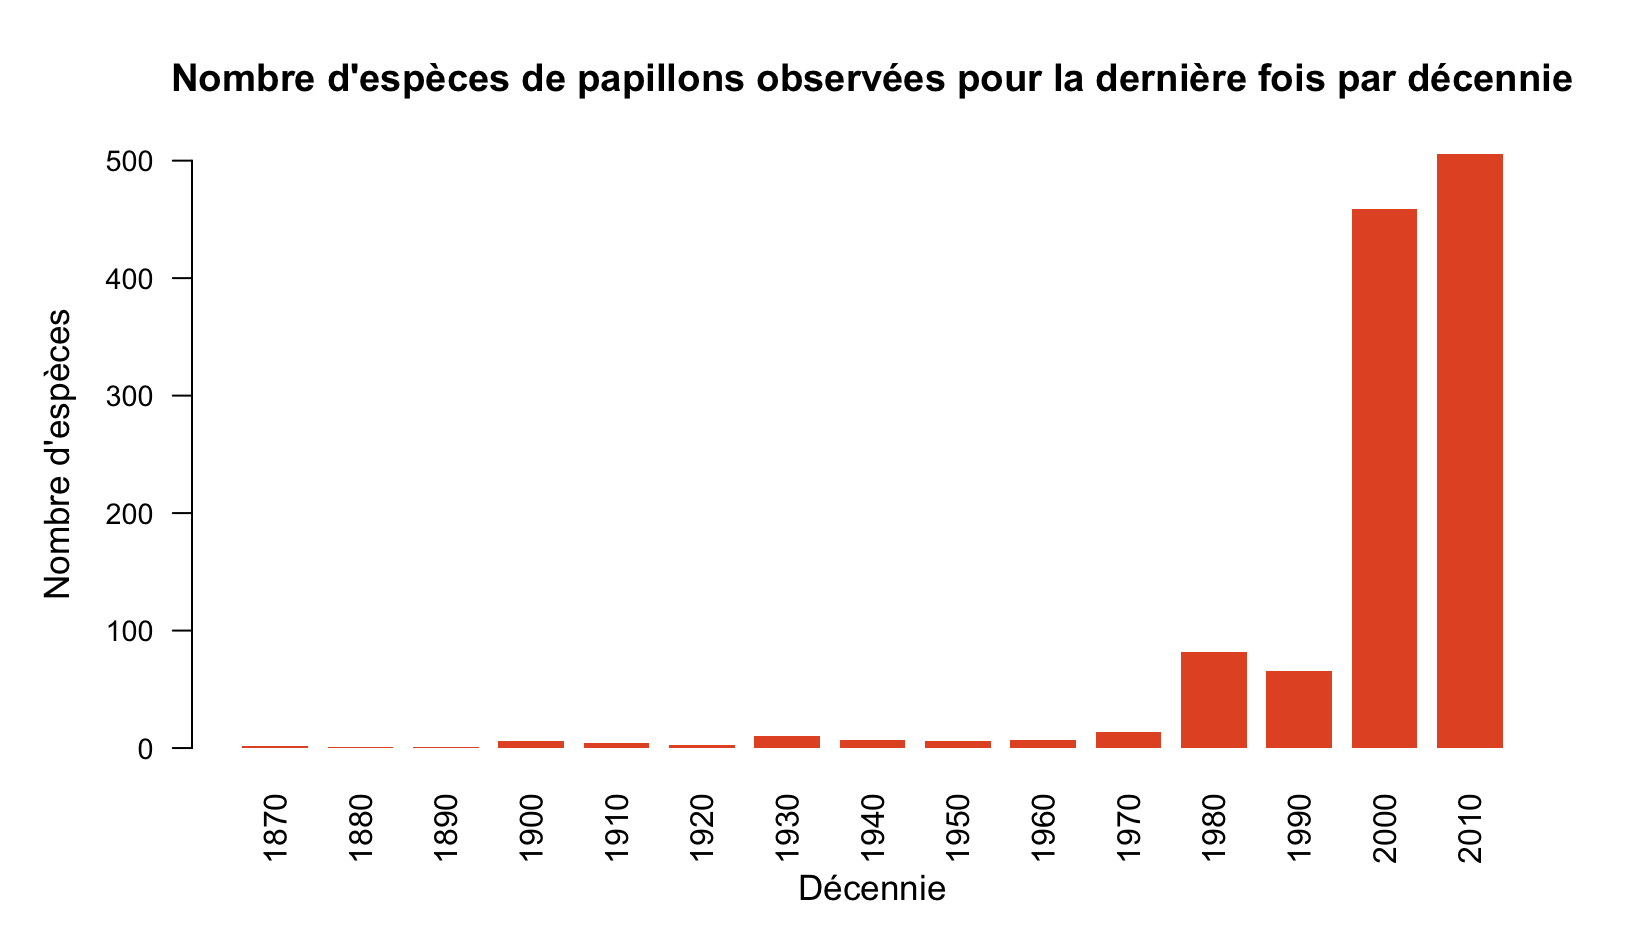
\includegraphics[width=\textwidth,height=0.4\textheight]{fig_nb_esp_obs_derniere_fois}
\caption{Nombre d'espèces de papillons observées pour la dernière fois
par décennie au Québec}
\end{figure}

\begin{figure}
\centering
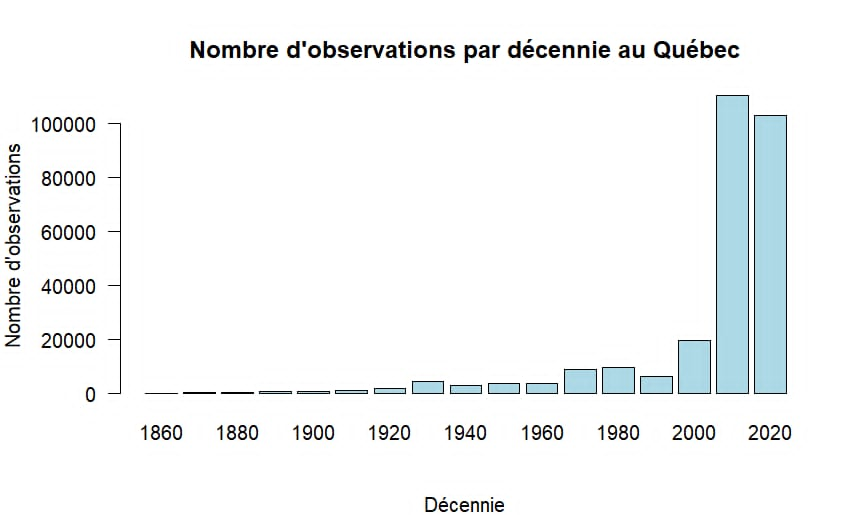
\includegraphics[width=\textwidth,height=0.4\textheight]{nb_obs_par_decennie.jpeg}
\caption{Nombre d'observations par décennie au Québec}
\end{figure}

\begin{figure}
\centering
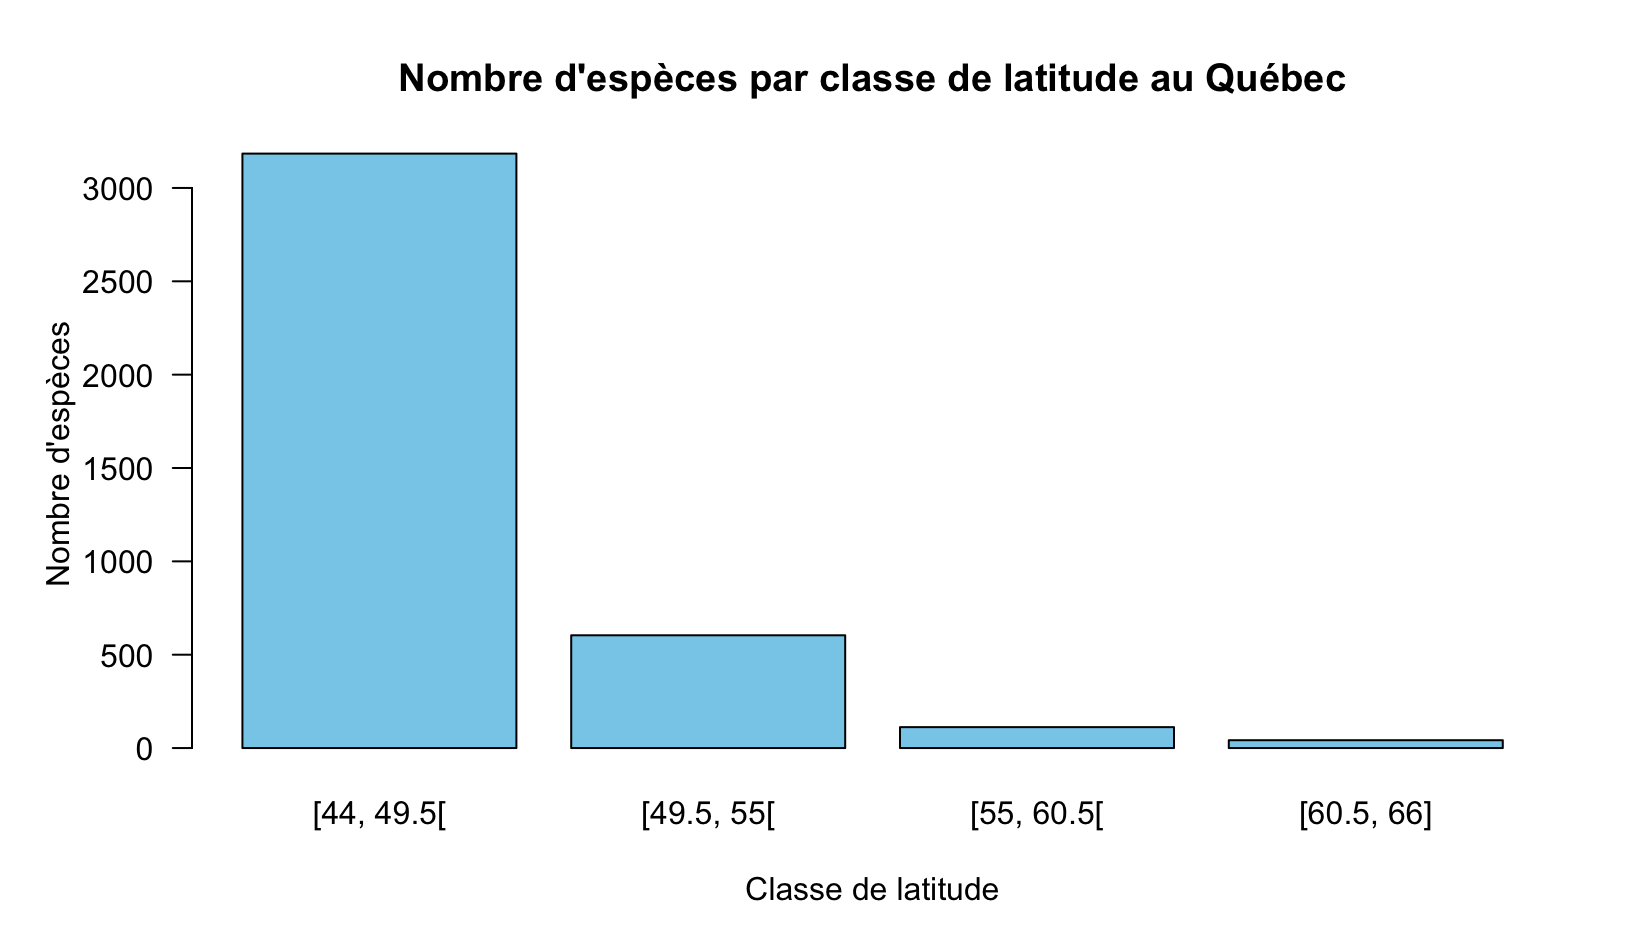
\includegraphics[width=\textwidth,height=0.4\textheight]{nb_esp_par_latitude.png}
\caption{Nombre d'espèces de papillons par classe de latitude au Québec}
\end{figure}

\begin{figure}
\centering
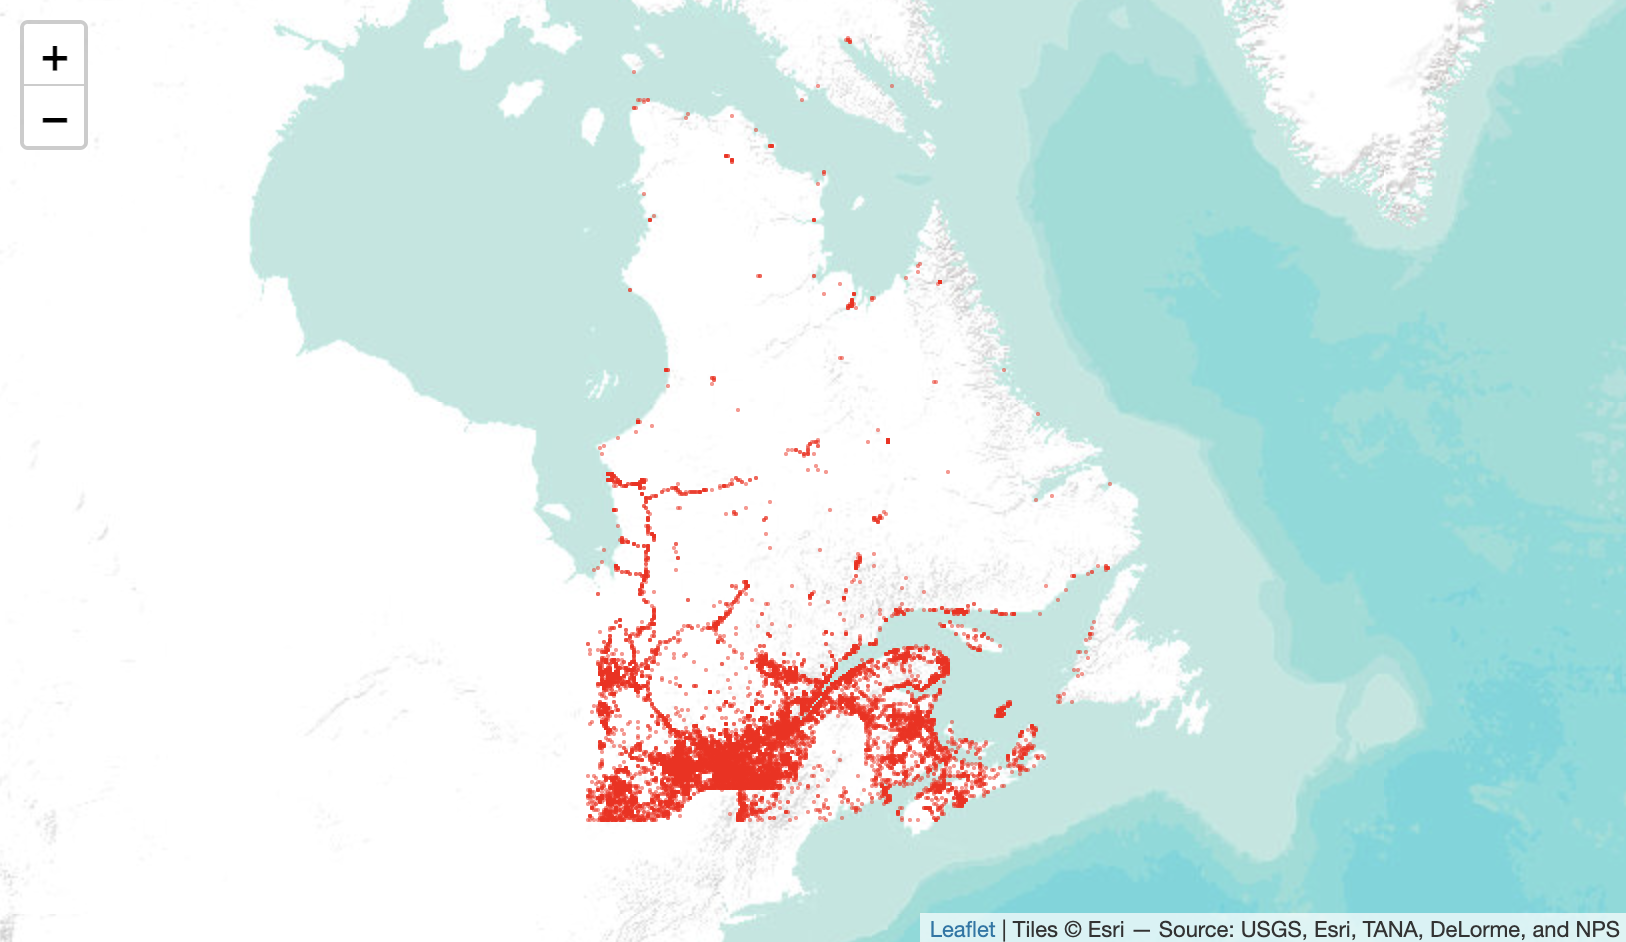
\includegraphics[width=\textwidth,height=0.4\textheight]{Carte.png}
\caption{Carte des observations}
\end{figure}

\begin{center}\rule{0.5\linewidth}{0.5pt}\end{center}

\section{Discussion}\label{discussion}

\subsection{Quantité d'espèces recensées pour la dernière
fois}\label{quantituxe9-despuxe8ces-recensuxe9es-pour-la-derniuxe8re-fois}

On peut voir sur la figure 3, le nombre d'espèces aperçues pour la
dernière fois pendant une certaine décennie. Le fait qu'une espèce a été
vue pour la dernière fois ne signifie pas nécessairement qu'elle est
disparue. Il est toutefois probable que son abondance soit moindre à
partir de ce moment. Si celle-ci est moins abondante, les chances
qu'elle soit observée le sont aussi.

Il ne faut pas oublier que ces chiffres sont nuancés par l'effort
d'échantillonnage, illustré par la figure 4. L'abondance d'espèces dans
les dernières décennies est expliquée, en partie, par l'effort
d'échantillonnage. Un échantillonnage plus intensif nous amène à inclure
des espèces rares, parfois observées une seule fois, mais considérées
comme si cette observation était leur dernière. Cependant, il est
logique de voir que le nombre d'espèces en déclin augmente dans les
dernières décennies. Avec l'augmentation des conséquences de l'activité
humaine, l'abondance de lépidoptères aux États-Unis a diminué de 22\%
entre 2000 et 2020 {[}1{]}. On observe cette diminution pendant les
mêmes années de nos données.

\subsection{Quantité d'espèces recensées pour la première fois dans
notre base de
données}\label{quantituxe9-despuxe8ces-recensuxe9es-pour-la-premiuxe8re-fois-dans-notre-base-de-donnuxe9es}

La figure 2 montre la quantité d'espèces de lépidoptères recensées pour
la première fois. Nous n'avons pas retiré les observations qui ont eu
lieu pour la première fois pendant la première décennie, en 1860,
puisqu'il n'y a eu que 6 observations de 4 espèces. Nous les avons
conservées puisque cela ne faussera pas nos analyses en montrant un
chiffre très grand de « nouvelles espèces » au début de
l'échantillonnage. Encore une fois, ces chiffres sont nuancés par
l'effort d'échantillonnage, qu'on peut voir avec la figure 4. Il est
normal d'observer plus d'espèces pour la première fois lorsqu'il y a
plus de données qui ont été prises. Ce graphique reflète plus
l'amélioration de la science et des techniques d'échantillonnage que
l'état des espèces. Même en 2000, c'était l'avis de R. F. Chapman que
l'entomologie a énormément progressé avec la technologie et que les
questions qu'on se pose aujourd'hui, étaient inconcevable il y a
quelques décennies {[}9{]}.

Il serait très étonnant de découvrir des centaines de nouvelles espèces
de papillons au Québec alors qu'aux États-Unis, entre 2000 et 2020, des
chercheurs ont démontré que 33\% des espèces de lépidoptères ont décliné
significativement, par rapport à 3\% des espèces qui ont montré une
tendance à la hausse {[}1{]}. Cependant, il est logique que des espèces
qui n'avaient pas encore été décrites au début de la récolte de données
soient observées dans les décennies suivantes. Même aujourd'hui, on
estime qu'il y a encore entre 1 et 4 millions d'espèces d'insectes non
décrites {[}10{]}.

\subsection{Latitudes où se retrouvent le plus d'espèces de
lépidoptères}\label{latitudes-ouxf9-se-retrouvent-le-plus-despuxe8ces-de-luxe9pidoptuxe8res}

Comme illustré sur la figure 5, la plupart des espèces de lépidoptères
se trouvent au sud du Québec. L'augmentation de la température à cet
endroit augmente la valeur adaptative des papillons. Les pertes de
chaleur sont réduites, leur permettant de consacrer plus de temps à la
recherche de nourriture. De plus, un hiver plus chaud augmente leurs
chances de survie {[}11{]}.

Une autre étude au Canada a relevé que la richesse des papillons est
plus élevée dans les zones où il y a plus d'activité humaine. En effet,
celle-ci est plus élevée au sud du Québec (à basses latitudes). Il faut
cependant savoir qu'à l'intérieur de ces zones, la diversité est
inversement proportionnelle à l'intensité de l'activité humaine
{[}12{]}. La perte et la fragmentation d'habitat sont, entre autres, des
impacts humains nuisibles aux papillons. Convertir des forêts en champs
peut être bénéfique, mais l'agriculture intensive et les pesticides qui
y sont liés sont dommageables {[}11{]}.

\subsection{Localisation des
observations}\label{localisation-des-observations}

Une partie des données a été faite avec la science citoyenne. Cela
pourrait expliquer pourquoi beaucoup d'observations sont au sud, donc où
la population est plus dense. Bien que la science citoyenne apporte de
la main-d'œuvre à faible coût, plusieurs biais y sont associés.
Certaines espèces ou certaines régions peuvent être plus reportées,
uniquement car elles sont préférées par les observateurs. {[}13{]}. La
capacité à reporter une observation (exemple à la prendre en photo)
exerce également une influence {[}13{]}.

\begin{center}\rule{0.5\linewidth}{0.5pt}\end{center}

\section{References}\label{references}

\begin{itemize}
\item
  {[}1{]} C. B. Edwards et al., « Rapid butterfly declines across the
  United States during the 21st century », Science, vol.~387, no 6738,
  p.~1090‑1094, mars 2025, doi: 10.1126/science.adp4671.
\item
  {[}2{]} R Core Team., R: A language and environment for statistical
  computing. (2024). R Foundation for Statistical Computing. {[}En
  ligne{]}. Disponible sur: \url{https://www.R-project.org/}
\item
  {[}3{]} T. Barrett et al., \emph{data.table: Extension of
  \texttt{data.frame}}. R package version 1.17.0,. (2025). {[}En
  ligne{]}. Disponible sur:
  \url{https://CRAN.R-project.org/package=data.table}
\item
  {[}4{]} H. Wickham, R. François, L. Henry, K. Müller, et D. Vaughan,
  dplyr: A Grammar of Data Manipulation\_. R package version 1.1.4.
  (2023). {[}En ligne{]}. Disponible sur:
  \url{https://CRAN.R-project.org/package=dplyr}
\item
  {[}5{]} K. Müller, H. Wickham, D. James, et S. Falcon, RSQLite: SQLite
  Interface for R\_. R package version 2.3.9,. (2024). {[}En ligne{]}.
  Disponible sur: \url{https://CRAN.R-project.org/package=RSQLite}
\item
  {[}6{]} J. Cheng, B. Schloerke, B. Karambelkar, et Y. Xie, leaflet:
  Create Interactive Web Maps with the JavaScript « Leaflet » Library\_.
  R package version 2.2.2,. (2024). {[}En ligne{]}. Disponible sur:
  \url{https://CRAN.R-project.org/package=leaflet}
\item
  {[}7{]} H. Wickham, ggplot2: Elegant Graphics for Data Analysis.
  Springer-Verlag New York,. (2016). {[}En ligne{]}. Disponible sur:
  \url{https://ggplot2.tidyverse.org}
\item
  {[}8{]} W. Landau, The targets R package: a dynamic Make-like
  function-oriented pipeline toolkit for reproducibility and
  high-performance computing. Journal of Open Source Software, 6(57),
  2959,. (2021). {[}En ligne{]}. Disponible sur:
  \url{https://doi.org/10.21105/joss.02959}
\item
  {[}9{]} R. F. Chapman, « Entomology in the Twentieth Century », Annual
  Review of Entomology, vol.~45, no Volume 45, 2000, p.~261‑285, janv.
  2000, doi: 10.1146/annurev.ento.45.1.261.
\item
  {[}10{]} M. J. Costello, S. Wilson, et B. Houlding, « Predicting Total
  Global Species Richness Using Rates of Species Description and
  Estimates of Taxonomic Effort », Systematic Biology, vol.~61, no 5,
  p.~871, oct. 2012, doi: 10.1093/sysbio/syr080.
\item
  {[}11{]} P. White et J. T. Kerr, « Contrasting spatial and temporal
  global change impacts on butterfly species richness during the 20th
  century », Ecography, vol.~29, no 6, p.~908‑918, 2006, doi:
  10.1111/j.2006.0906-7590.04685.x.
\item
  {[}12{]} P. J. T. White et J. T. Kerr, « Human impacts on
  environment--diversity relationships: evidence for biotic
  homogenization from butterfly species richness patterns », Global
  Ecology and Biogeography, vol.~16, no 3, p.~290‑299, 2007, doi:
  10.1111/j.1466-8238.2007.00298.x.
\item
  {[}13{]} O. Arazy, K. Kaplan-Mintz, D. Malkinson, et Y. Nagar, « A
  local community on a global collective intelligence platform: A case
  study of individual preferences and collective bias in ecological
  citizen science », PLOS ONE, vol.~19, no 8, p.~e0308552, août 2024,
  doi: 10.1371/journal.pone.0308552.
\end{itemize}

\bibliography{Libidopterebiblio.bib}


\end{document}
